\chapter{An Empirical Study \label{chap:empirical_study}}

Excluding Dixon's factorization method, all attacks analyzed so far exploit
some peculiarities of a candidate RSA public key $\angular{N, e}$ in order to
recover the private exponent.
Summarizingly:
\begin{itemize}
  \item Pollard's $p-1$ attack works only if the predecessor of any of
    the two primes factorizing the public modulus is composed of very small
    prime powers;
  \item  Williams' $p+1$ attack works under similar conditions - on the
    predecessor or the successor of any of the two primes ;
  \item Fermat's factorization is valuable whenever the two primes $p$ and $q$
    are really close to each other;
  \item Pollard's $\rho$ method is best whenever one of the two primes is
    strictly lower than the other;
  \item Wiener's attack is guaranteed to work on small private exponents.
\end{itemize}
Dixon's factorization method instead, being a general-purpose factorization
algorithm, can be employed to \emph{measure} the strength of a RSA
keypair: the more relations (satisfying \ref{eq:dixon:fermat_revisited}) are
found, the less it is assumed to be resistant.

Given these hypothesis, it has been fairly easy to produce valid RSA candidate
keys that can be broken using the above attacks. They have been used to assert
the correctness of the implementation.

On the top of that, there has been a chance to test the software under real
conditions: we downloaded the SSL keys (if any) of the top one million visited
websites, and survey them with the just developed software. This not only gave
us the opportunity to survey the degree of security on which the internet is
grounded today, but also led to a deeper understanding of the capacities and limits of
the most widespread libraries offering crypto nowadays.

\vfill
\section{To skim off the dataset}

What has been most scandalous above all was to discover that more than
\strong{half} of the most visited websites do \strong{not} provide SSL
connection over port 443 - reserved for HTTPS according to IANA
\cite{iana:ports}.
To put it in numbers, we are talking about $533, 000$ websites either
unresolved or unreachable in $10$ seconds.
As a side note for this, many websites (like \texttt{baidu.com} or
\texttt{qq.com}) keep a TCP connection open without writing anything to the
channel, requiring us to adopt a combination of non-blocking socket with the
\texttt{select()} system call in order to drop any empty communication.
It would be interesting to investigate more on these facts, asking ourselves how
many of those unsuccessful connections are actually wanted from the server, and
how many dropped for censorship reasons; there is enough room for another
project.

Of the remaining $450,000$ keys, $21$ were using different ciphers than RSA. All
others represent the dataset upon which we worked on.

\section{To count}

Once all valuable certificate informations have been stored inside a database,
almost any query can be performed to get a statistically valuable measure of
degree of magnitude to which some conditions are satisfied. What follows now is
a list of commented examples that we believe are relevant parameters for
understanding of how badly internet is configured today.


\begin{figure}[H]
  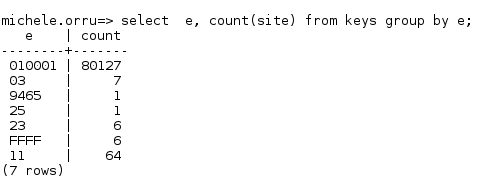
\includegraphics[width=0.7\textwidth]{e_count.png}
\end{figure}

The most prolific number we see here, $65537$ in hexadecimal, is the fourth
Fermat number and no other than the largest known prime of the form $2^{2^n} +
1$. Due to its composition, it has been advised by NIST as default public
exponent, and successfully implemented in most software, such as \openssl\!.

Sadly, a negligible number of websites is using low public exponents,
which makes the RSA key vulnerable to Coppersmith's attack; though, this
topic goes beyond the scope of this research and hence has not been analyzed
further.

\begin{figure}[H]
  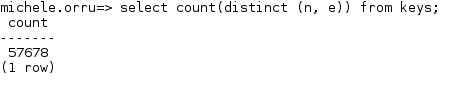
\includegraphics[width=0.7\textwidth]{n_count.png}
\end{figure}

What is interesting to see here is that an enormous portion of our dataset
shared the same public key, pushing down the number of expected keys of one
order of magnitude. Reasons for this are mostly practical: it is extremely
frequent to have blogs hosted on third-party services such as ``Blogspot'' or
``Wordpress'' which always provide the same X.509 certificate, as they belong to
an unique organization.
Though improbable, it is even possible that exists a millesimal portion of
different websites sharing the same public key due to a
bad cryptographically secure random number generator, and therefore also the
same private key. Such a case has been already investigated in \cite{ron:whit}.

\begin{figure}[H]
  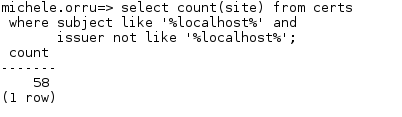
\includegraphics[width=0.6\textwidth]{localhost_certs.png}
\end{figure}

Here we go. A suprisingly consistent number of websites provides certificates
filled with dummy, wrong, or even testing informations.\\
Some do have non-printable bytes in the \emph{common name} field.\\
Some are certified from authorities. \\
Some are even gonvernmental entities.

\begin{figure}[H]
  \includegraphics[width=0.9\textwidth]{bits_count.png}
\end{figure}

According to \cite{nist:keylen_transitions} \S 3, table $2$, all RSA keys of
bitlength less than $1024$ are to be considered deprecated at the end of $2013$
and shall no more be issued since the beginning of this year. Not differently
from the above results, the remark has been globally adopted, yet still with a
few exceptions: around a dozen of non-self-signed certificates with a 1024 RSA
key appears to have been issued in 2014.


\section{The proof and the concept}

At the time of this writing, we have collected the output of only two
mathematical tests performed in the university cluster.

\paragraph{Wiener.} The attack described in chapter \ref{chap:wiener} was the
first employed, being the fastest one above all others. Recalling the different
public exponents we probed (discussed in the previous sections), we expected all
private exponents to be $>  \rfrac{1}{3}\sqrt[4]{N}$; there is still the
possibility that the attack works, but there is no guarantee.
For what concerns our tests, we found no weak keys that could be recovered using
Wiener's attack.

\paragraph{GCD.} On the wave of \cite{ron:whit}, whe attempted also to perform
the $\gcd$ of every possible pair of dinstinct public modulus present in the
dataset. In contrast to our expectations, this test led to no prime factor
leaked, for any key pair. We have reasons to believe this depends on the
relatively small size of our dataset, with respect to the one used in
\cite{ron:whit}.



\chapter{Conclusions \label{conclusions}}

Everytime we surf the web, we share our communication channel with lots of
entities around the globe. End-to-end encryption protocols such as TLS can
provide the security  properties that we often take as granted, like
\emph{confidentiality}, \emph{integrity}, and \emph{authenticity}; though,
these holds only if we \emph{trust} the authorities certifying the end entity.

%% Wax Taylor - Que Sera
There is this mindless thinking that whenever we see that small lock icon in the
browser's url bar, somebody is telling us the connection is safe.
There is some authority out there telling what to do, and we should be thinking
more about what these authorities are and what they are doing.
This issue is no more a technical problem, but instead is becoming more and more
a social and political problem.
It is our responsability as citzens to do something about that.


%%% Local Variables:
%%% mode: latex
%%% TeX-master: "question_authority"
%%% End:
